\chapter{Introduzione}

\section{Intro al Corso}

\paragraph{Parole chiave:}

\begin{itemize}
  \item Web Apps. 
  \item Mission Critical.
  \item DevOps.
  \item Cloud Native.

\end{itemize}

\dfn{Mission Critical Applications}{
  Un'applicazione o sistema le cui operazioni sono fondamentali per una compagnia o un'istituzione.
}

\clm{}{}{
  \begin{itemize}
    \item Enfasi sui requisiti non funzionali: i requisiti funzionali sono la baseline, ma ci si aspetta di più per rimanere competitivi. 
    \item Da non confondere con life critical: non muore nessuno.
  \end{itemize}
}

\dfn{Enterprise Application Integration (EAI)}{
  Tutto l'insieme di pratiche architetturali, tecnologie, patterns, frameworks e strumenti che consentono la comunicazione e la condivisione tra diverse applicazioni nella stessa organizzazione.
}

\paragraph{Si ha enfasi sull'infrastruttura:} 
\begin{itemize}
  \item \fancyglitter{Data Integration:} combinare dati da più moduli diversi (coinvolge database). 
  \item \fancyglitter{Process Integration:} le interazioni tra più moduli. 
  \item \fancyglitter{Functional Integration:} si vuole fornire una nuova funzionalità sfruttando funzionalità già esistenti.
\end{itemize}
\pagebreak
\subsection{Esempio e Requisiti Non Funzionali}

\begin{figure}[h]
    \centering
    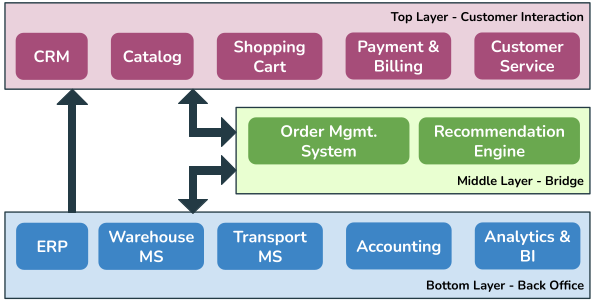
\includegraphics[scale=0.7]{01/crm.png}
    \caption{Esempio di e-commerce.}
\end{figure}

\paragraph{Commento dell'esempio:}

\begin{itemize}
  \item Ci sono tre livelli: 
    \begin{itemize}
      \item Top Layer: moduli che si rivolgono al cliente.
      \item Middle Layer: gestione della comunicazione tra cliente e azienda. 
      \item Bottom Layer: moduli interni aziendali.
    \end{itemize}
\end{itemize}

\paragraph{Requisiti non funzionali:}

\begin{itemize}
  \item High availability/zero downtime: l'applicativo deve essere sempre o quasi sempre disponibile. 
  \item Affidabilità: in caso di interruzione di workflow si deve far sì che non ci siano stati danni (e.g. un'interruzione durante una transazione). 
  \item Consistenza dei dati. 
  \item Integrità dei dati. 
  \item Low latency: per avere una buona performance, tutto deve essere fluido. 
  \item Scalabilità.
  \item Sicurezza. 
  \item Resilienza: capacità di reagire agli errori. 
  \item Mantenibilità: quanto un pezzo di software sia mantenibile o riutilizzabile.
  \item Osservabilità: per comprendere eventuali problemi in un sistema distribuito. 
  \item Auditability: le verifiche di qualità fatte su software\footnote{Meglio visto in "Etica, Società e Privacy".}.
\end{itemize}

\subsection{Panoramica Storica}

\dfn{Waterfall}{
  Le metodologie a cascata\footnote{Viste a "Sviluppo delle Applicazioni Software".} sono metodologie in cui ci sono fasi ben distinte e separate tra loro.
}

\nt{È un modello prevedibile, ma lento a gestire i cambiamenti.}

\clm{}{}{
  \begin{itemize}
    \item Software on the shelf: una volta acquistato è proprio. 
    \item Software custom: prodotto su richiesta, ha bisogno di tutto un servizio di manutenzione. 
  \end{itemize}
}

\dfn{Lean}{
  Metodologie nate negli anni '50 alla Toyota, verranno applicate al software dagli anni '90. Si basa su tre principi: 
  \begin{itemize}
    \item Muda\footnote{JOJO'S Reference} (waste): si deve stare sui requisiti, non mettere troppe funzioni non necessarie. 
    \item Mura (unevenness): è necessaria consinstenza per aumentare la prevedibilità.  
    \item Muri (overburden): non sovraccaricare le persone o le macchine. Non progettare software utilizzando strumenti greedy di risorse.
  \end{itemize} 
}

\nt{Lo strumento fondamentale è il \fancyglitter{kanban}: la lavagna, per organizzare il lavoro.}

\dfn{Siloed}{
  Organizzazione aziendale a silos: si comunica poco e male. CI sono 4 gruppi: 
  \begin{itemize}
    \item BA Team: relazioni con gli stakeholders, requisiti, specifiche, documentazione. 
    \item Dev Team: programma e fa un minimo di unit testing. 
    \item Test Team: testa e decide se il sistema è pronto. 
    \item Ops Team: si occupa del deployement.
  \end{itemize}
}





